\documentclass[12pt,a4paper]{article}
\usepackage{amsmath,amssymb,amsfonts}
\usepackage{graphicx}
\usepackage{tikz}
\usepackage{float}
\usepackage{hyperref}
\usepackage{xcolor}
\usepackage{tcolorbox}
\usepackage{enumitem}
\usepackage{calc}

\usetikzlibrary{arrows,shapes,positioning,shadows,trees,decorations.pathreplacing,calc}

\hypersetup{
    colorlinks=true,
    linkcolor=blue,
    filecolor=magenta,
    urlcolor=cyan,
}

\title{3. Reinforcement Learning: Markov Decision Processes}
\author{Reinforcement Learning Notes}


\begin{document}

\maketitle
\tableofcontents
\newpage

\section{Introduction to Markov Decision Processes}

\subsection{Motivation and Context}

Markov Decision Processes (MDPs) provide the formal mathematical framework for modeling reinforcement learning problems where an agent interacts with an environment through sequential decision-making. MDPs extend upon simpler paradigms like multi-armed bandits and contextual bandits by introducing:

\begin{itemize}
    \item A fully specified notion of state
    \item State transitions influenced by agent actions
    \item Long-term consequences of decisions
\end{itemize}

In a multi-armed bandit problem, only the immediate reward is considered, with no concept of state. In contextual bandits, while rewards depend on states, the actions do not influence future states. MDPs provide the next evolutionary step, where an agent's actions both affect immediate rewards and influence the probability distribution of future states.

\subsection{The Agent-Environment Interface}

The standard agent-environment interface in reinforcement learning is formalized through MDPs:

\begin{figure}[H]
\centering
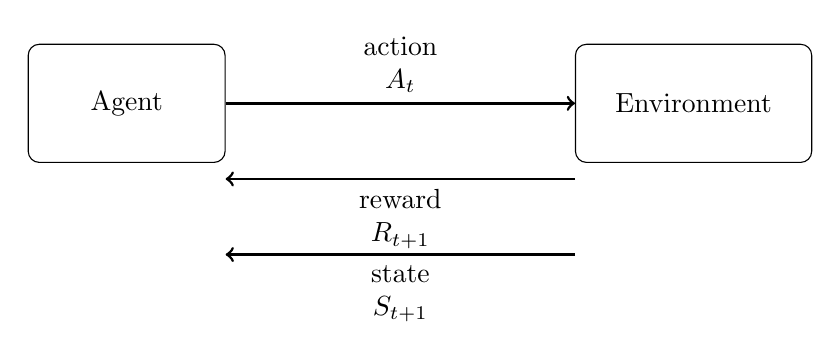
\begin{tikzpicture}[scale=1.2]
    % Boxes for Agent and Environment
    \node[draw, rounded corners, minimum width=2.5cm, minimum height=1.5cm] (agent) at (0,0) {Agent};
    \node[draw, rounded corners, minimum width=3cm, minimum height=1.5cm] (env) at (6,0) {Environment};
    
    % Action arrow from Agent to Environment
    \draw[->, line width=1pt] (agent.east) -- node[above, align=center] {action\\$A_t$} (env.west);
    
    % Reward and State arrows from Environment to Agent
    \draw[->, line width=1pt] (env.west |- 0,-0.8) -- node[below, align=center] {reward\\$R_{t+1}$} (agent.east |- 0,-0.8);
    \draw[->, line width=1pt] (env.west |- 0,-1.6) -- node[below, align=center] {state\\$S_{t+1}$} (agent.east |- 0,-1.6);
\end{tikzpicture}
\caption{The agent-environment interaction in reinforcement learning (Sutton \& Barto)}
\end{figure}

The interaction proceeds as follows:
\begin{itemize}
    \item At each time step $t$, the agent observes the current state $S_t \in \mathcal{S}$
    \item Based on this state, the agent selects an action $A_t \in \mathcal{A}(S_t)$
    \item The environment responds with a reward $R_{t+1} \in \mathcal{R}$ and transitions to a new state $S_{t+1}$
    \item This creates a sequence of states, actions, and rewards: $S_0, A_0, R_1, S_1, A_1, R_2, S_2, \ldots$
\end{itemize}

The goal of the agent is to select actions that maximize the expected cumulative reward over time.

\section{Components of MDPs}

\subsection{States, Actions, Rewards, and Transitions}

A Markov Decision Process is defined by four essential components:

\begin{enumerate}
    \item \textbf{States} ($\mathcal{S}$): The set of all possible states of the environment. A state $s \in \mathcal{S}$ provides all relevant information needed for decision-making. The state at time $t$ is denoted $S_t$.
    
    \item \textbf{Actions} ($\mathcal{A}$): The set of all possible actions the agent can take. For each state $s$, the agent can choose from a set of available actions $\mathcal{A}(s)$. The action at time $t$ is denoted $A_t$.
    
    \item \textbf{Transitions}: The state transition probability function $p(s'|s,a)$ defines the dynamics of the environment. It specifies the probability of transitioning to state $s'$ given that the agent was in state $s$ and took action $a$.
    
    \item \textbf{Rewards} ($\mathcal{R}$): The reward function $r(s,a)$ defines the immediate reward received after taking action $a$ in state $s$. The reward at time $t+1$ (after taking action $A_t$ in state $S_t$) is denoted $R_{t+1}$.
\end{enumerate}

\subsection{The Markov Property}

The defining characteristic of MDPs is the Markov property, which states that the future is independent of the past given the present. Formally, a state $S_t$ is Markov if and only if:

\begin{equation}
P(S_{t+1}=s', R_{t+1}=r | S_t, A_t, R_t, S_{t-1}, A_{t-1}, \ldots, R_1, S_0, A_0) = P(S_{t+1}=s', R_{t+1}=r | S_t, A_t)
\end{equation}

\begin{tcolorbox}[title=Notation Overview]
\begin{itemize}
    \item $P(S_{t+1}=s', R_{t+1}=r | S_t, A_t, \ldots)$ - The probability of transitioning to state $s'$ and receiving reward $r$ given the entire history
    \item $P(S_{t+1}=s', R_{t+1}=r | S_t, A_t)$ - The probability of transitioning to state $s'$ and receiving reward $r$ given only the current state and action
    \item $S_t$ - The state at time step $t$
    \item $A_t$ - The action taken at time step $t$
    \item $R_t$ - The reward received at time step $t$
\end{itemize}
\end{tcolorbox}

The Markov property implies that the current state captures all relevant information from the history of the process. This is a crucial assumption that simplifies the decision-making problem while still capturing the essential dynamics of many real-world sequential decision problems.

\section{Formal MDP Definition}

\subsection{Mathematical Notation}

A finite Markov Decision Process is formally defined as a 5-tuple $(\mathcal{S}, \mathcal{A}, p, r, \gamma)$ where:

\begin{itemize}
    \item $\mathcal{S}$ is a finite set of states
    \item $\mathcal{A}$ is a finite set of actions
    \item $p: \mathcal{S} \times \mathcal{A} \times \mathcal{S} \times \mathcal{R} \rightarrow [0, 1]$ is the state transition probability function
    \item $r: \mathcal{S} \times \mathcal{A} \rightarrow \mathbb{R}$ is the reward function
    \item $\gamma \in [0, 1]$ is the discount factor
\end{itemize}

The dynamics of the environment are fully specified by the joint probability distribution:

\begin{equation}
p(s',r|s,a) = P(S_t = s', R_t = r|S_{t-1} = s, A_{t-1} = a)
\end{equation}

\begin{tcolorbox}[title=Notation Overview]
\begin{itemize}
    \item $p(s',r|s,a)$ - The probability of transitioning to state $s'$ and receiving reward $r$, given that the agent was in state $s$ and took action $a$
    \item $P(S_t = s', R_t = r|S_{t-1} = s, A_{t-1} = a)$ - The probability that the state at time $t$ is $s'$ and the reward is $r$, given that the state at time $t-1$ was $s$ and the action taken was $a$
    \item $S_t$ - The state at time step $t$
    \item $R_t$ - The reward received at time step $t$
    \item $A_t$ - The action taken at time step $t$
\end{itemize}
\end{tcolorbox}

From this joint probability function, we can derive other important quantities:

\subsection{State Transition Probabilities}

The state transition probabilities are derived from the joint probability by summing over all possible rewards:

\begin{equation}
p(s'|s,a) = \sum_{r \in \mathcal{R}} p(s',r|s,a)
\end{equation}

\begin{tcolorbox}[title=Notation Overview]
\begin{itemize}
    \item $p(s'|s,a)$ - The probability of transitioning to state $s'$ given state $s$ and action $a$
    \item $p(s',r|s,a)$ - The joint probability of transitioning to state $s'$ and receiving reward $r$, given state $s$ and action $a$
    \item $\mathcal{R}$ - The set of all possible rewards
\end{itemize}
\end{tcolorbox}

\subsection{Expected Reward Functions}

There are several ways to define the expected reward, each useful in different contexts:

\begin{equation}
r(s,a) = \mathbb{E}[R_t|S_{t-1}=s, A_{t-1}=a] = \sum_{r \in \mathcal{R}} r \sum_{s' \in \mathcal{S}} p(s',r|s,a)
\end{equation}

\begin{tcolorbox}[title=Notation Overview]
\begin{itemize}
    \item $r(s,a)$ - The expected reward when taking action $a$ in state $s$
    \item $\mathbb{E}[\cdot]$ - The expected value operator
    \item $R_t$ - The reward at time $t$
    \item $S_{t-1}$ - The state at time $t-1$
    \item $A_{t-1}$ - The action taken at time $t-1$
    \item $p(s',r|s,a)$ - The joint probability of transitioning to state $s'$ and receiving reward $r$, given state $s$ and action $a$
    \item $\mathcal{S}$ - The set of all possible states
    \item $\mathcal{R}$ - The set of all possible rewards
\end{itemize}
\end{tcolorbox}

\subsection{Example of Expected Reward Calculation}

Let's illustrate the calculation of the expected reward with a simple example:

Consider a tiny MDP with:
\begin{itemize}
    \item 2 states: $s_1$ and $s_2$
    \item 1 action: $a$
    \item 2 possible rewards: 0 and 1
\end{itemize}

The transition probabilities are defined as:
\begin{itemize}
    \item $p(s_1, 0|s_1, a) = 0.3$ (30\% chance of staying in $s_1$ with reward 0)
    \item $p(s_2, 0|s_1, a) = 0.2$ (20\% chance of moving to $s_2$ with reward 0)
    \item $p(s_1, 1|s_1, a) = 0.1$ (10\% chance of staying in $s_1$ with reward 1)
    \item $p(s_2, 1|s_1, a) = 0.4$ (40\% chance of moving to $s_2$ with reward 1)
\end{itemize}

To calculate the expected reward $r(s_1, a)$, we apply the formula:
\begin{align*}
r(s_1, a) &= \sum_{r \in \mathcal{R}} r \sum_{s' \in \mathcal{S}} p(s', r|s_1, a) \\
&= 0 \cdot \sum_{s' \in \mathcal{S}} p(s', 0|s_1, a) + 1 \cdot \sum_{s' \in \mathcal{S}} p(s', 1|s_1, a) \\
&= 0 \cdot (p(s_1, 0|s_1, a) + p(s_2, 0|s_1, a)) + 1 \cdot (p(s_1, 1|s_1, a) + p(s_2, 1|s_1, a)) \\
&= 0 \cdot (0.3 + 0.2) + 1 \cdot (0.1 + 0.4) \\
&= 0 \cdot 0.5 + 1 \cdot 0.5 \\
&= 0.5
\end{align*}

This example shows how the inner sum (over $s'$) collects probabilities for the same reward across different next states, and the outer sum (over $r$) adds up the weighted rewards.

We can also define the expected reward for state-action-next-state triples:

\begin{equation}
r(s,a,s') = \mathbb{E}[R_t|S_{t-1}=s, A_{t-1}=a, S_t=s'] = \sum_{r \in \mathcal{R}} r \frac{p(s',r|s,a)}{p(s'|s,a)}
\end{equation}

\begin{tcolorbox}[title=Notation Overview]
\begin{itemize}
    \item $r(s,a,s')$ - The expected reward when transitioning from state $s$ to state $s'$ via action $a$
    \item $\mathbb{E}[\cdot]$ - The expected value operator
    \item $R_t$ - The reward at time $t$
    \item $S_{t-1}$ - The state at time $t-1$
    \item $A_{t-1}$ - The action taken at time $t-1$
    \item $S_t$ - The state at time $t$
    \item $p(s',r|s,a)$ - The joint probability of transitioning to state $s'$ and receiving reward $r$, given state $s$ and action $a$
    \item $p(s'|s,a)$ - The probability of transitioning to state $s'$ given state $s$ and action $a$
    \item $\mathcal{R}$ - The set of all possible rewards
\end{itemize}
\end{tcolorbox}

\subsection{MDP Constraints}

For a valid MDP, the following constraints must be satisfied:

\begin{enumerate}
    \item $\sum_{s' \in \mathcal{S}} \sum_{r \in \mathcal{R}} p(s',r|s,a) = 1$ for all $s \in \mathcal{S}$ and $a \in \mathcal{A}(s)$
    \item $p(s',r|s,a) \geq 0$ for all $s, s' \in \mathcal{S}$, $r \in \mathcal{R}$, and $a \in \mathcal{A}(s)$
\end{enumerate}

These constraints ensure that $p(s',r|s,a)$ is a valid probability distribution.

\section{Policy Definition}

\subsection{Formalization of Policies}

A policy is a mapping from states to probabilities of selecting each possible action. Formally, a policy $\pi$ is defined as:

\begin{equation}
\pi(a|s) = P(A_t = a | S_t = s)
\end{equation}

\begin{tcolorbox}[title=Notation Overview]
\begin{itemize}
    \item $\pi(a|s)$ - The probability of selecting action $a$ in state $s$ under policy $\pi$
    \item $P(A_t = a | S_t = s)$ - The probability that the agent selects action $A_t = a$ when in state $S_t = s$
    \item $A_t$ - The action taken at time step $t$
    \item $S_t$ - The state at time step $t$
\end{itemize}
\end{tcolorbox}

\subsection{Types of Policies}

Policies can be categorized based on their stochasticity:

\begin{enumerate}
    \item \textbf{Deterministic Policies}: For each state, exactly one action is selected with probability 1, and all other actions have probability 0. A deterministic policy can be written as $\pi(s) = a$, indicating that action $a$ is always selected in state $s$.
    
    \item \textbf{Stochastic Policies}: Actions are selected according to a probability distribution. Stochastic policies are useful for exploration and for solving problems with partial observability or non-deterministic dynamics.
\end{enumerate}

\subsection{Stationary vs. Non-Stationary Policies}

Another categorization of policies is based on their time-dependence:

\begin{enumerate}
    \item \textbf{Stationary Policies}: The policy does not change over time. The mapping from states to action probabilities remains constant regardless of the time step.
    
    \item \textbf{Non-Stationary Policies}: The policy changes over time. The mapping from states to action probabilities depends on the time step.
\end{enumerate}

In most reinforcement learning contexts, we focus on finding optimal stationary policies, as they are simpler and often sufficient for solving MDPs.

\subsection{Examples of Policies}

Several common policy types used in reinforcement learning include:

\begin{itemize}
    \item \textbf{Greedy Policy}: Always selects the action with the highest estimated value:
    \begin{equation}
    \pi(a|s) = 
    \begin{cases}
    1 & \text{if } a = \arg\max_{a'} Q(s,a') \\
    0 & \text{otherwise}
    \end{cases}
    \end{equation}
    
    \item \textbf{$\epsilon$-Greedy Policy}: Selects the best action most of the time, but occasionally explores:
    \begin{equation}
    \pi(a|s) = 
    \begin{cases}
    1 - \epsilon + \frac{\epsilon}{|\mathcal{A}(s)|} & \text{if } a = \arg\max_{a'} Q(s,a') \\
    \frac{\epsilon}{|\mathcal{A}(s)|} & \text{otherwise}
    \end{cases}
    \end{equation}
    
    \item \textbf{Softmax Policy}: Selects actions with probabilities proportional to their estimated values:
    \begin{equation}
    \pi(a|s) = \frac{e^{Q(s,a)/\tau}}{\sum_{a'} e^{Q(s,a')/\tau}}
    \end{equation}
    where $\tau$ is a temperature parameter controlling exploration.
\end{itemize}

\begin{tcolorbox}[title=Notation Overview]
\begin{itemize}
    \item $\pi(a|s)$ - The probability of selecting action $a$ in state $s$ under policy $\pi$
    \item $Q(s,a)$ - The estimated value of taking action $a$ in state $s$
    \item $\arg\max_{a'}$ - The action that maximizes the given function
    \item $\epsilon$ - A small probability for random exploration
    \item $|\mathcal{A}(s)|$ - The number of possible actions in state $s$
    \item $\tau$ - Temperature parameter in softmax, controlling exploration (higher values increase randomness)
\end{itemize}
\end{tcolorbox}

\section{Episodic vs. Continuing Tasks}

\subsection{Episodic Tasks}

Episodic tasks are those with a clear endpoint or terminal state:

\begin{itemize}
    \item Each episode starts from an initial state and ends when a terminal state is reached
    \item Examples include board games (chess, Go), where games have a definite beginning and end
    \item The interaction breaks naturally into subsequences called "episodes"
    \item Each episode ends in a special terminal state, often with different rewards for different outcomes
\end{itemize}

In episodic tasks, we denote the set of all non-terminal states as $\mathcal{S}$ and the set of all states, including the terminal state, as $\mathcal{S}^+$.

\subsection{Continuing Tasks}

Continuing tasks are those that go on indefinitely without a natural endpoint:

\begin{itemize}
    \item The agent-environment interaction does not break into episodes and continues without limit
    \item Examples include ongoing process control, perpetual robot operation, or stock portfolio management
    \item There is no terminal state, so the agent must learn to perform well over an indefinite horizon
\end{itemize}

\subsection{Unified Notation}

To unify the notation for both episodic and continuing tasks, we can use a single formulation by considering episodic tasks as continuing tasks with a special absorbing terminal state that transitions only to itself with a reward of zero.

\begin{figure}[H]
\centering
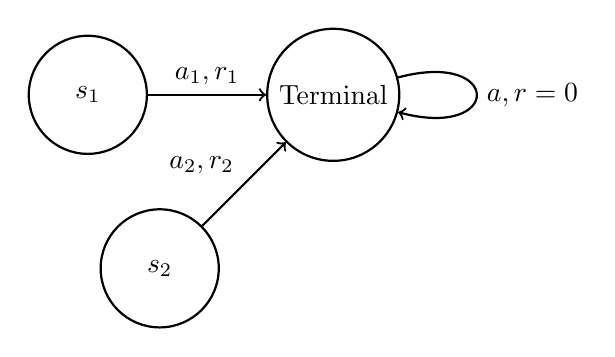
\begin{tikzpicture}[node distance=1.5cm, auto, thick]
    % Terminal state
    \node[draw,circle,minimum size=1.5cm] (terminal) {Terminal};
    
    % Self-loop
    \draw[->] (terminal) to [loop right] node {$a, r=0$} (terminal);
    
    % Incoming transitions (simplified)
    \node[draw,circle,minimum size=1.5cm, left=of terminal] (s1) {$s_1$};
    \node[draw,circle,minimum size=1.5cm, below left=of terminal] (s2) {$s_2$};
    
    \draw[->] (s1) -- node {$a_1, r_1$} (terminal);
    \draw[->] (s2) -- node {$a_2, r_2$} (terminal);
\end{tikzpicture}
\caption{Representation of a terminal state in an episodic task}
\end{figure}

This unification allows us to treat both episodic and continuing tasks within the same mathematical framework.

\section{Discounted Future Return}

\subsection{Definition of Return}

In reinforcement learning, the agent aims to maximize not just immediate rewards but the cumulative reward over time. The return is the function of reward sequence that the agent seeks to maximize.

For a continuing task, the simplest formulation would be the sum of rewards:
\begin{equation}
G_t = R_{t+1} + R_{t+2} + R_{t+3} + \ldots
\end{equation}

\begin{tcolorbox}[title=Notation Overview]
\begin{itemize}
    \item $G_t$ - The return at time step $t$
    \item $R_{t+k}$ - The reward received $k$ steps after time $t$
\end{itemize}
\end{tcolorbox}

However, this sum could be infinite for continuing tasks, making it unsuitable as an optimization criterion.

\subsection{Discounting}

To address this issue, we introduce discounting, which reduces the importance of future rewards:

\begin{equation}
G_t = R_{t+1} + \gamma R_{t+2} + \gamma^2 R_{t+3} + \ldots = \sum_{k=0}^{\infty} \gamma^k R_{t+k+1}
\end{equation}

\begin{tcolorbox}[title=Notation Overview]
\begin{itemize}
    \item $G_t$ - The discounted return at time step $t$
    \item $R_{t+k+1}$ - The reward received $k+1$ steps after time $t$
    \item $\gamma$ - The discount factor, $0 \leq \gamma \leq 1$
    \item $\sum_{k=0}^{\infty}$ - The sum over all future time steps
\end{itemize}
\end{tcolorbox}

The discount factor $\gamma$ determines how much the agent values future rewards:
\begin{itemize}
    \item $\gamma$ close to 0: Myopic evaluation, immediate rewards are strongly preferred
    \item $\gamma$ close to 1: Far-sighted evaluation, future rewards are valued almost as much as immediate ones
\end{itemize}

\subsection{Reasons for Discounting}

There are several reasons to use discounting:

\begin{enumerate}
    \item \textbf{Mathematical Convenience}: Ensures the sum is finite for continuing tasks, provided $\gamma < 1$
    \item \textbf{Uncertainty about the Future}: Future rewards are more uncertain, which may justify valuing them less
    \item \textbf{Alignment with Human Preferences}: People often prefer immediate rewards to delayed ones
    \item \textbf{Avoidance of Infinite Returns}: Without discounting, optimal policies might not exist for continuing tasks
\end{enumerate}

\subsection{Episodic Returns}

For episodic tasks with a terminal time step $T$, the return can be defined as:

\begin{equation}
G_t = \sum_{k=0}^{T-t-1} \gamma^k R_{t+k+1}
\end{equation}

\begin{tcolorbox}[title=Notation Overview]
\begin{itemize}
    \item $G_t$ - The return at time step $t$
    \item $R_{t+k+1}$ - The reward received $k+1$ steps after time $t$
    \item $\gamma$ - The discount factor, $0 \leq \gamma \leq 1$
    \item $T$ - The final time step of the episode
    \item $T-t-1$ - The number of remaining steps in the episode after time $t$
\end{itemize}
\end{tcolorbox}

\subsection{Unified Return Formulation}

To unify notation for both episodic and continuing tasks, we can use:

\begin{equation}
G_t = \sum_{k=t+1}^{T} \gamma^{k-t-1} R_k
\end{equation}

\begin{tcolorbox}[title=Notation Overview]
\begin{itemize}
    \item $G_t$ - The return at time step $t$
    \item $R_k$ - The reward received at time step $k$
    \item $\gamma$ - The discount factor, $0 \leq \gamma \leq 1$
    \item $T$ - The final time step (could be $\infty$ for continuing tasks)
    \item $k-t-1$ - The number of time steps between receiving reward $R_k$ and time $t$
\end{itemize}
\end{tcolorbox}

This formulation handles both episodic tasks (where $T$ is finite) and continuing tasks (where $T = \infty$). Note that for continuing tasks, $\gamma < 1$ is required to ensure the sum is finite.

\subsection{Recursive Relationship for Return}

The return has a useful recursive relationship:

\begin{equation}
G_t = R_{t+1} + \gamma G_{t+1}
\end{equation}

\begin{tcolorbox}[title=Notation Overview]
\begin{itemize}
    \item $G_t$ - The return at time step $t$
    \item $R_{t+1}$ - The immediate reward received after time $t$
    \item $\gamma$ - The discount factor, $0 \leq \gamma \leq 1$
    \item $G_{t+1}$ - The return at time step $t+1$
\end{itemize}
\end{tcolorbox}

This recursive relationship is fundamental to many reinforcement learning methods, particularly those based on bootstrapping.

\section{Value Functions}

\subsection{State-Value Function}

The state-value function $v_\pi(s)$ represents how good it is for an agent to be in a particular state $s$ when following policy $\pi$. Formally, it is defined as the expected return starting from state $s$ and following policy $\pi$ thereafter:

\begin{equation}
v_\pi(s) = \mathbb{E}_\pi[G_t | S_t = s]
\end{equation}

\begin{tcolorbox}[title=Notation Overview]
\begin{itemize}
    \item $v_\pi(s)$ - The state-value function for policy $\pi$
    \item $\mathbb{E}_\pi[\cdot]$ - The expected value when following policy $\pi$
    \item $G_t$ - The return at time step $t$
    \item $S_t$ - The state at time step $t$
\end{itemize}
\end{tcolorbox}

We can expand this definition using the recursive relationship for the return:

\begin{equation}
v_\pi(s) = \mathbb{E}_\pi[R_{t+1} + \gamma G_{t+1} | S_t = s]
\end{equation}

\begin{tcolorbox}[title=Notation Overview]
\begin{itemize}
    \item $v_\pi(s)$ - The state-value function for policy $\pi$
    \item $\mathbb{E}_\pi[\cdot]$ - The expected value when following policy $\pi$
    \item $R_{t+1}$ - The immediate reward
    \item $\gamma$ - The discount factor, $0 \leq \gamma \leq 1$
    \item $G_{t+1}$ - The return at time step $t+1$
    \item $S_t$ - The state at time step $t$
\end{itemize}
\end{tcolorbox}

\subsection{Action-Value Function}

The action-value function $q_\pi(s,a)$ represents how good it is to take a specific action $a$ in state $s$ when following policy $\pi$ thereafter. Formally:

\begin{equation}
q_\pi(s,a) = \mathbb{E}_\pi[G_t | S_t = s, A_t = a]
\end{equation}

\begin{tcolorbox}[title=Notation Overview]
\begin{itemize}
    \item $q_\pi(s,a)$ - The action-value function for policy $\pi$
    \item $\mathbb{E}_\pi[\cdot]$ - The expected value when following policy $\pi$
    \item $G_t$ - The return at time step $t$
    \item $S_t$ - The state at time step $t$
    \item $A_t$ - The action taken at time step $t$
\end{itemize}
\end{tcolorbox}

\subsection{Relationship Between Value Functions}

The state-value and action-value functions are related by:

\begin{equation}
v_\pi(s) = \sum_{a} \pi(a|s) q_\pi(s, a)
\end{equation}

\begin{tcolorbox}[title=Notation Overview]
\begin{itemize}
    \item $v_\pi(s)$ - The state-value function for policy $\pi$
    \item $\pi(a|s)$ - The probability of taking action $a$ in state $s$ under policy $\pi$
    \item $q_\pi(s,a)$ - The action-value function for policy $\pi$
    \item $\sum_{a}$ - The sum over all possible actions in state $s$
\end{itemize}
\end{tcolorbox}

This equation shows that the value of a state equals the expected value of the actions that might be taken in that state, weighted by their probability under policy $\pi$.

Conversely, the action-value function can be expressed in terms of the state-value function:

\begin{equation}
q_\pi(s, a) = \sum_{s', r} p(s', r|s, a) [r + \gamma v_\pi(s')]
\end{equation}

\begin{tcolorbox}[title=Notation Overview]
\begin{itemize}
    \item $q_\pi(s,a)$ - The action-value function for policy $\pi$
    \item $p(s', r|s, a)$ - The probability of transitioning to state $s'$ and receiving reward $r$, given state $s$ and action $a$
    \item $r$ - The immediate reward
    \item $\gamma$ - The discount factor, $0 \leq \gamma \leq 1$
    \item $v_\pi(s')$ - The state-value function for policy $\pi$ at the next state $s'$
    \item $\sum_{s', r}$ - The sum over all possible next states and rewards
\end{itemize}
\end{tcolorbox}

This equation shows that the value of taking action $a$ in state $s$ equals the expected immediate reward plus the discounted value of the next state.

\subsection{The Bellman Equation for State-Value Function}

The Bellman equation expresses the recursive relationship in value functions. For the state-value function:

\begin{equation}
v_\pi(s) = \sum_{a} \pi(a|s) \sum_{s',r} p(s',r|s,a) [r + \gamma v_\pi(s')]
\end{equation}

\begin{tcolorbox}[title=Notation Overview]
\begin{itemize}
    \item $v_\pi(s)$ - The state-value function for policy $\pi$
    \item $\pi(a|s)$ - The probability of taking action $a$ in state $s$ under policy $\pi$
    \item $p(s',r|s,a)$ - The probability of transitioning to state $s'$ and receiving reward $r$, given state $s$ and action $a$
    \item $r$ - The immediate reward
    \item $\gamma$ - The discount factor, $0 \leq \gamma \leq 1$
    \item $v_\pi(s')$ - The state-value function for policy $\pi$ at the next state $s'$
    \item $\sum_{a}$ - The sum over all possible actions in state $s$
    \item $\sum_{s',r}$ - The sum over all possible next states and rewards
\end{itemize}
\end{tcolorbox}

The Bellman equation states that the value of a state equals the expected return for taking an action according to policy $\pi$, which consists of the immediate reward plus the discounted value of the next state.

\subsection{The Bellman Equation for Action-Value Function}

Similarly, the Bellman equation for the action-value function is:

\begin{equation}
q_\pi(s,a) = \sum_{s',r} p(s',r|s,a) \left[r + \gamma \sum_{a'} \pi(a'|s') q_\pi(s',a') \right]
\end{equation}

\begin{tcolorbox}[title=Notation Overview]
\begin{itemize}
    \item $q_\pi(s,a)$ - The action-value function for policy $\pi$
    \item $p(s',r|s,a)$ - The probability of transitioning to state $s'$ and receiving reward $r$, given state $s$ and action $a$
    \item $r$ - The immediate reward
    \item $\gamma$ - The discount factor, $0 \leq \gamma \leq 1$
    \item $\pi(a'|s')$ - The probability of taking action $a'$ in the next state $s'$ under policy $\pi$
    \item $q_\pi(s',a')$ - The action-value function for policy $\pi$ at the next state-action pair $(s', a')$
    \item $\sum_{s',r}$ - The sum over all possible next states and rewards
    \item $\sum_{a'}$ - The sum over all possible actions in the next state $s'$
\end{itemize}
\end{tcolorbox}

\subsection{Backup Diagrams for Bellman Equations}

Backup diagrams provide a graphical representation of the Bellman equations, illustrating how values are propagated from future states back to the current state.

\begin{figure}[H]
\centering
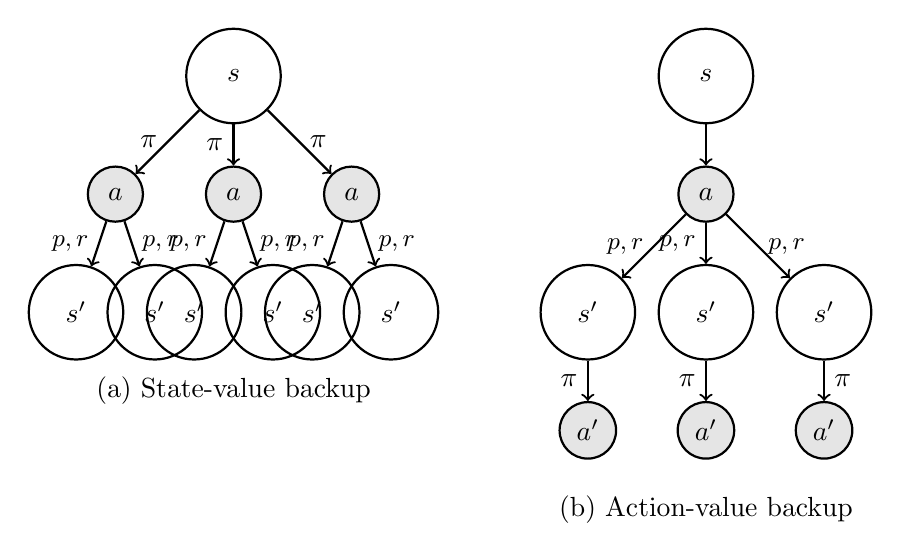
\begin{tikzpicture}[scale=1.0, transform shape, thick]
    % State-value backup
    \node[draw, circle, minimum size=1.2cm] (s) at (0,0) {$s$};
    \node[draw, circle, fill=gray!20, minimum size=0.7cm] (a1) at (-1.5,-1.5) {$a$};
    \node[draw, circle, fill=gray!20, minimum size=0.7cm] (a2) at (0,-1.5) {$a$};
    \node[draw, circle, fill=gray!20, minimum size=0.7cm] (a3) at (1.5,-1.5) {$a$};
    \node[draw, circle, minimum size=1.2cm] (s11) at (-2,-3) {$s'$};
    \node[draw, circle, minimum size=1.2cm] (s12) at (-1,-3) {$s'$};
    \node[draw, circle, minimum size=1.2cm] (s21) at (-0.5,-3) {$s'$};
    \node[draw, circle, minimum size=1.2cm] (s22) at (0.5,-3) {$s'$};
    \node[draw, circle, minimum size=1.2cm] (s31) at (1,-3) {$s'$};
    \node[draw, circle, minimum size=1.2cm] (s32) at (2,-3) {$s'$};
    
    % Connect nodes
    \draw[->] (s) -- node[left] {$\pi$} (a1);
    \draw[->] (s) -- node[left] {$\pi$} (a2);
    \draw[->] (s) -- node[right] {$\pi$} (a3);
    
    \draw[->] (a1) -- node[left, font=\small] {$p,r$} (s11);
    \draw[->] (a1) -- node[right, font=\small] {$p,r$} (s12);
    \draw[->] (a2) -- node[left, font=\small] {$p,r$} (s21);
    \draw[->] (a2) -- node[right, font=\small] {$p,r$} (s22);
    \draw[->] (a3) -- node[left, font=\small] {$p,r$} (s31);
    \draw[->] (a3) -- node[right, font=\small] {$p,r$} (s32);
    
    % Labels
    \node at (0,-4) {(a) State-value backup};
    
    % Action-value backup
    \node[draw, circle, minimum size=1.2cm] (s_q) at (6,0) {$s$};
    \node[draw, circle, fill=gray!20, minimum size=0.7cm] (a_q) at (6,-1.5) {$a$};
    \node[draw, circle, minimum size=1.2cm] (s1_q) at (4.5,-3) {$s'$};
    \node[draw, circle, minimum size=1.2cm] (s2_q) at (6,-3) {$s'$};
    \node[draw, circle, minimum size=1.2cm] (s3_q) at (7.5,-3) {$s'$};
    \node[draw, circle, fill=gray!20, minimum size=0.7cm] (a1_q) at (4.5,-4.5) {$a'$};
    \node[draw, circle, fill=gray!20, minimum size=0.7cm] (a2_q) at (6,-4.5) {$a'$};
    \node[draw, circle, fill=gray!20, minimum size=0.7cm] (a3_q) at (7.5,-4.5) {$a'$};
    
    % Connect nodes
    \draw[->] (s_q) -- (a_q);
    
    \draw[->] (a_q) -- node[left, font=\small] {$p,r$} (s1_q);
    \draw[->] (a_q) -- node[left, font=\small] {$p,r$} (s2_q);
    \draw[->] (a_q) -- node[right, font=\small] {$p,r$} (s3_q);
    
    \draw[->] (s1_q) -- node[left] {$\pi$} (a1_q);
    \draw[->] (s2_q) -- node[left] {$\pi$} (a2_q);
    \draw[->] (s3_q) -- node[right] {$\pi$} (a3_q);
    
    % Labels
    \node at (6,-5.5) {(b) Action-value backup};
\end{tikzpicture}
\caption{Backup diagrams for (a) the state-value function $v_\pi$ and (b) the action-value function $q_\pi$}
\end{figure}

In these diagrams:
\begin{itemize}
    \item Solid circles represent states
    \item Open circles represent actions
    \item The root node at the top represents the state or state-action pair being evaluated
    \item The branches show possible trajectories
    \item Nodes are traversed from top to bottom when following trajectories
    \item Values are backed up from bottom to top when computing the value function
\end{itemize}

\section{Optimal Policies and Value Functions}

\subsection{Definition of Optimal Policies}

A policy $\pi$ is defined as better than or equal to a policy $\pi'$ if its expected return is greater than or equal to that of $\pi'$ for all states:

\begin{equation}
\pi \geq \pi' \iff v_\pi(s) \geq v_{\pi'}(s) \text{ for all } s \in \mathcal{S}
\end{equation}

\begin{tcolorbox}[title=Notation Overview]
\begin{itemize}
    \item $\pi \geq \pi'$ - Policy $\pi$ is better than or equal to policy $\pi'$
    \item $v_\pi(s)$ - The state-value function for policy $\pi$
    \item $v_{\pi'}(s)$ - The state-value function for policy $\pi'$
    \item $\mathcal{S}$ - The set of all possible states
\end{itemize}
\end{tcolorbox}

There is always at least one policy that is better than or equal to all other policies, called an optimal policy, denoted $\pi_*$. All optimal policies share the same optimal state-value function, $v_*$:

\begin{equation}
v_*(s) = \max_{\pi} v_\pi(s) \text{ for all } s \in \mathcal{S}
\end{equation}

\begin{tcolorbox}[title=Notation Overview]
\begin{itemize}
    \item $v_*(s)$ - The optimal state-value function
    \item $\max_{\pi}$ - The maximum over all possible policies
    \item $v_\pi(s)$ - The state-value function for policy $\pi$
    \item $\mathcal{S}$ - The set of all possible states
\end{itemize}
\end{tcolorbox}

They also share the same optimal action-value function, $q_*$:

\begin{equation}
q_*(s,a) = \max_{\pi} q_\pi(s,a) \text{ for all } s \in \mathcal{S}, a \in \mathcal{A}(s)
\end{equation}

\begin{tcolorbox}[title=Notation Overview]
\begin{itemize}
    \item $q_*(s,a)$ - The optimal action-value function
    \item $\max_{\pi}$ - The maximum over all possible policies
    \item $q_\pi(s,a)$ - The action-value function for policy $\pi$
    \item $\mathcal{S}$ - The set of all possible states
    \item $\mathcal{A}(s)$ - The set of actions available in state $s$
\end{itemize}
\end{tcolorbox}

\subsection{The Bellman Optimality Equations}

The Bellman optimality equations characterize the optimal value functions:

\begin{equation}
v_*(s) = \max_a \sum_{s',r} p(s',r|s,a) [r + \gamma v_*(s')]
\end{equation}

\begin{tcolorbox}[title=Notation Overview]
\begin{itemize}
    \item $v_*(s)$ - The optimal state-value function
    \item $\max_a$ - The maximum over all actions $a \in \mathcal{A}(s)$
    \item $p(s',r|s,a)$ - The probability of transitioning to state $s'$ and receiving reward $r$, given state $s$ and action $a$
    \item $r$ - The immediate reward
    \item $\gamma$ - The discount factor, $0 \leq \gamma \leq 1$
    \item $v_*(s')$ - The optimal state-value function at the next state $s'$
    \item $\sum_{s',r}$ - The sum over all possible next states and rewards
\end{itemize}
\end{tcolorbox}

And for the action-value function:

\begin{equation}
q_*(s,a) = \sum_{s',r} p(s',r|s,a) [r + \gamma \max_{a'} q_*(s',a')]
\end{equation}

\begin{tcolorbox}[title=Notation Overview]
\begin{itemize}
    \item $q_*(s,a)$ - The optimal action-value function
    \item $p(s',r|s,a)$ - The probability of transitioning to state $s'$ and receiving reward $r$, given state $s$ and action $a$
    \item $r$ - The immediate reward
    \item $\gamma$ - The discount factor, $0 \leq \gamma \leq 1$
    \item $\max_{a'}$ - The maximum over all actions $a' \in \mathcal{A}(s')$
    \item $q_*(s',a')$ - The optimal action-value function at the next state-action pair $(s', a')$
    \item $\sum_{s',r}$ - The sum over all possible next states and rewards
\end{itemize}
\end{tcolorbox}

\subsection{Backup Diagrams for Bellman Optimality Equations}

\begin{figure}[H]
\centering
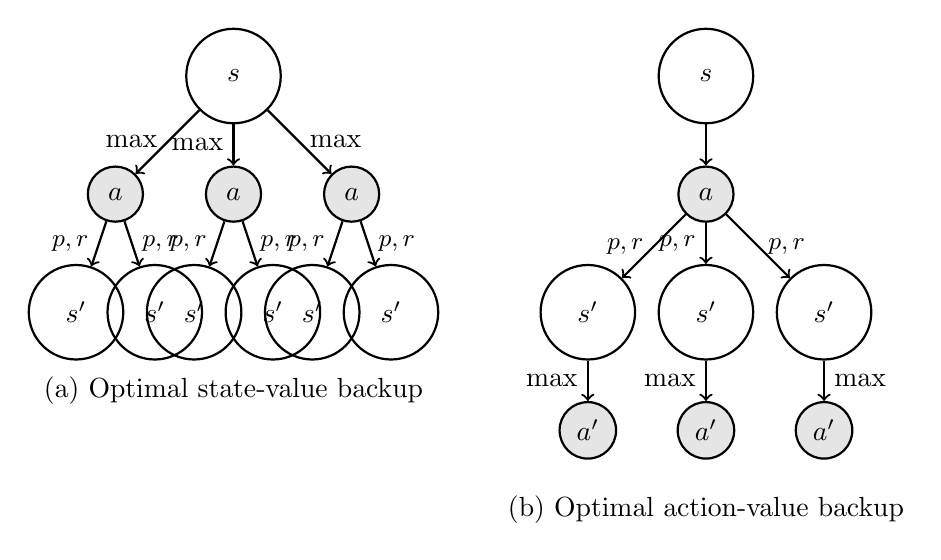
\begin{tikzpicture}[scale=1.0, transform shape, thick]
    % State-value backup
    \node[draw, circle, minimum size=1.2cm] (s) at (0,0) {$s$};
    \node[draw, circle, fill=gray!20, minimum size=0.7cm] (a1) at (-1.5,-1.5) {$a$};
    \node[draw, circle, fill=gray!20, minimum size=0.7cm] (a2) at (0,-1.5) {$a$};
    \node[draw, circle, fill=gray!20, minimum size=0.7cm] (a3) at (1.5,-1.5) {$a$};
    \node[draw, circle, minimum size=1.2cm] (s11) at (-2,-3) {$s'$};
    \node[draw, circle, minimum size=1.2cm] (s12) at (-1,-3) {$s'$};
    \node[draw, circle, minimum size=1.2cm] (s21) at (-0.5,-3) {$s'$};
    \node[draw, circle, minimum size=1.2cm] (s22) at (0.5,-3) {$s'$};
    \node[draw, circle, minimum size=1.2cm] (s31) at (1,-3) {$s'$};
    \node[draw, circle, minimum size=1.2cm] (s32) at (2,-3) {$s'$};
    
    % Connect nodes
    \draw[->] (s) -- node[left] {$\max$} (a1);
    \draw[->] (s) -- node[left] {$\max$} (a2);
    \draw[->] (s) -- node[right] {$\max$} (a3);
    
    \draw[->] (a1) -- node[left, font=\small] {$p,r$} (s11);
    \draw[->] (a1) -- node[right, font=\small] {$p,r$} (s12);
    \draw[->] (a2) -- node[left, font=\small] {$p,r$} (s21);
    \draw[->] (a2) -- node[right, font=\small] {$p,r$} (s22);
    \draw[->] (a3) -- node[left, font=\small] {$p,r$} (s31);
    \draw[->] (a3) -- node[right, font=\small] {$p,r$} (s32);
    
    % Labels
    \node at (0,-4) {(a) Optimal state-value backup};
    
    % Action-value backup
    \node[draw, circle, minimum size=1.2cm] (s_q) at (6,0) {$s$};
    \node[draw, circle, fill=gray!20, minimum size=0.7cm] (a_q) at (6,-1.5) {$a$};
    \node[draw, circle, minimum size=1.2cm] (s1_q) at (4.5,-3) {$s'$};
    \node[draw, circle, minimum size=1.2cm] (s2_q) at (6,-3) {$s'$};
    \node[draw, circle, minimum size=1.2cm] (s3_q) at (7.5,-3) {$s'$};
    \node[draw, circle, fill=gray!20, minimum size=0.7cm] (a1_q) at (4.5,-4.5) {$a'$};
    \node[draw, circle, fill=gray!20, minimum size=0.7cm] (a2_q) at (6,-4.5) {$a'$};
    \node[draw, circle, fill=gray!20, minimum size=0.7cm] (a3_q) at (7.5,-4.5) {$a'$};
    
    % Connect nodes
    \draw[->] (s_q) -- (a_q);
    
    \draw[->] (a_q) -- node[left, font=\small] {$p,r$} (s1_q);
    \draw[->] (a_q) -- node[left, font=\small] {$p,r$} (s2_q);
    \draw[->] (a_q) -- node[right, font=\small] {$p,r$} (s3_q);
    
    \draw[->] (s1_q) -- node[left] {$\max$} (a1_q);
    \draw[->] (s2_q) -- node[left] {$\max$} (a2_q);
    \draw[->] (s3_q) -- node[right] {$\max$} (a3_q);
    
    % Labels
    \node at (6,-5.5) {(b) Optimal action-value backup};
\end{tikzpicture}
\caption{Backup diagrams for (a) the optimal state-value function $v_*$ and (b) the optimal action-value function $q_*$}
\end{figure}

The key difference between these backup diagrams and those for $v_\pi$ and $q_\pi$ is the replacement of the policy distribution $\pi$ with the $\max$ operator, indicating that the agent selects the action that maximizes value.

\subsection{Deriving Optimal Policies}

Given the optimal value functions, it is straightforward to determine an optimal policy:

\begin{equation}
\pi_*(s) = \arg\max_a q_*(s,a)
\end{equation}

\begin{tcolorbox}[title=Notation Overview]
\begin{itemize}
    \item $\pi_*(s)$ - The optimal policy
    \item $\arg\max_a$ - The action that maximizes the given function
    \item $q_*(s,a)$ - The optimal action-value function
\end{itemize}
\end{tcolorbox}

Alternatively, using the state-value function:

\begin{equation}
\pi_*(s) = \arg\max_a \sum_{s',r} p(s',r|s,a) [r + \gamma v_*(s')]
\end{equation}

\begin{tcolorbox}[title=Notation Overview]
\begin{itemize}
    \item $\pi_*(s)$ - The optimal policy
    \item $\arg\max_a$ - The action that maximizes the given function
    \item $p(s',r|s,a)$ - The probability of transitioning to state $s'$ and receiving reward $r$, given state $s$ and action $a$
    \item $r$ - The immediate reward
    \item $\gamma$ - The discount factor, $0 \leq \gamma \leq 1$
    \item $v_*(s')$ - The optimal state-value function at the next state $s'$
    \item $\sum_{s',r}$ - The sum over all possible next states and rewards
\end{itemize}
\end{tcolorbox}

Any policy that is greedy with respect to the optimal value function(s) is an optimal policy. There may be multiple optimal policies that share the same optimal value function.

\section{Solving MDPs}

\subsection{Methods for Finding Optimal Policies}

Several methods can be used to solve MDPs:

\begin{enumerate}
    \item \textbf{Dynamic Programming (DP)}: When the MDP's dynamics (transition probabilities and reward function) are known, DP methods like policy iteration and value iteration can be used to compute optimal policies.
    
    \item \textbf{Monte Carlo (MC) Methods}: When the dynamics are unknown, MC methods use sample episodes to estimate values and improve the policy.
    
    \item \textbf{Temporal Difference (TD) Learning}: Combines ideas from DP and MC, updating value estimates based on other learned estimates without waiting for the end of an episode.
    
    \item \textbf{Model-Free Methods}: Methods like Q-learning and SARSA that learn directly from interaction with the environment without explicitly modeling its dynamics.
    
    \item \textbf{Model-Based Methods}: Methods that learn a model of the environment's dynamics and then use that model for planning.
\end{enumerate}

\subsection{The Generalized Policy Iteration Framework}

Many reinforcement learning methods follow a generalized policy iteration (GPI) framework, which alternates between policy evaluation and policy improvement:

\begin{figure}[H]
\centering
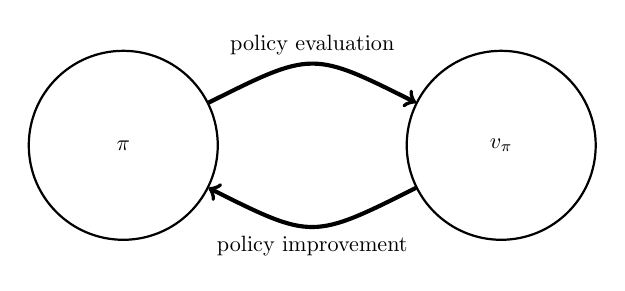
\begin{tikzpicture}[scale=0.8, transform shape, thick]
    % Circles for policy and value function
    \node[draw, circle, minimum size=3cm] (policy) at (0,0) {$\pi$};
    \node[draw, circle, minimum size=3cm] (value) at (6,0) {$v_\pi$};
    
    % Arrows
    \draw[->, line width=1.5pt] (policy) .. controls (3,1.5) .. node[above] {policy evaluation} (value);
    \draw[->, line width=1.5pt] (value) .. controls (3,-1.5) .. node[below] {policy improvement} (policy);
\end{tikzpicture}
\caption{The generalized policy iteration framework}
\end{figure}

\begin{itemize}
    \item \textbf{Policy Evaluation}: Compute the value function $v_\pi$ for the current policy $\pi$
    \item \textbf{Policy Improvement}: Improve the policy by making it greedy with respect to the current value function
    \item This process continues until convergence to the optimal policy and value function
\end{itemize}

Different methods vary in how they implement these two steps and how they interleave them.

\section{Example Applications of MDPs}

\subsection{Grid World Example}

A classic example of an MDP is the grid world problem:

\begin{figure}[H]
\centering
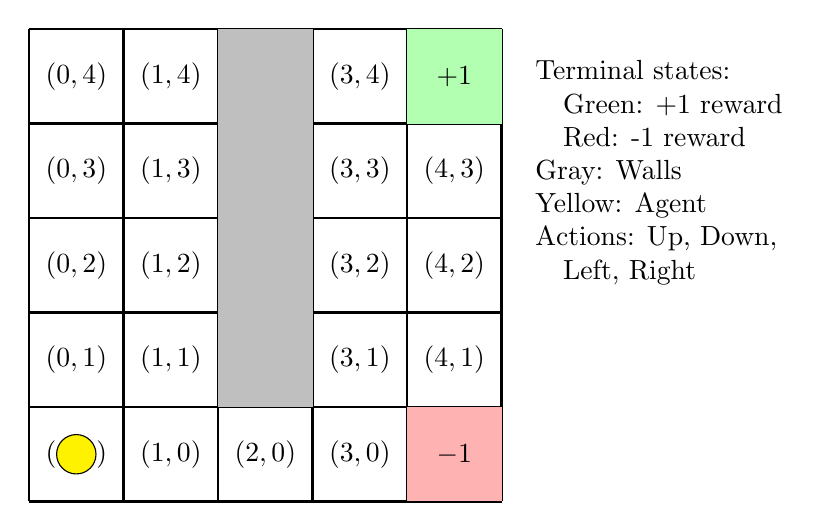
\begin{tikzpicture}[scale=0.8]
    % Draw grid
    \draw[step=1.5cm, line width=1pt] (0,0) grid (7.5,7.5);
    
    % Label grid positions
    \foreach \x in {0,1,2,3,4}
      \foreach \y in {0,1,2,3,4}
        \node at (1.5*\x+0.75, 1.5*\y+0.75) {$(\x,\y)$};
    
    % Terminal states
    \fill[green!30] (6,6) rectangle (7.5,7.5);
    \node at (6.75,6.75) {$+1$};
    
    \fill[red!30] (6,0) rectangle (7.5,1.5);
    \node at (6.75,0.75) {$-1$};
    
    % Walls
    \fill[gray!50] (3,1.5) rectangle (4.5,7.5);
    
    % Agent
    \node[circle, draw, fill=yellow, minimum size=0.5cm] at (0.75,0.75) {};
    
    % Legend
    \node[align=left] at (10,5) {
    Terminal states:\\
    \quad Green: +1 reward\\
    \quad Red: -1 reward\\
    Gray: Walls\\
    Yellow: Agent\\
    Actions: Up, Down,\\
    \quad Left, Right\\
    };
\end{tikzpicture}
\caption{Example grid world MDP}
\end{figure}

In this environment:
\begin{itemize}
    \item States are the grid positions $(x, y)$
    \item Actions are movements in four directions: up, down, left, right
    \item Transitions are deterministic (moving in a direction always results in the corresponding adjacent cell, unless blocked by a wall or grid boundary)
    \item Rewards are -1 for each step, except when reaching terminal states
    \item Terminal states have rewards of +1 (green) and -1 (red)
    \item The goal is to find the policy that maximizes the expected return (i.e., reach the green state with the minimum number of steps)
\end{itemize}

\subsection{Robot Navigation}

MDPs can model robot navigation problems:

\begin{figure}[H]
\centering
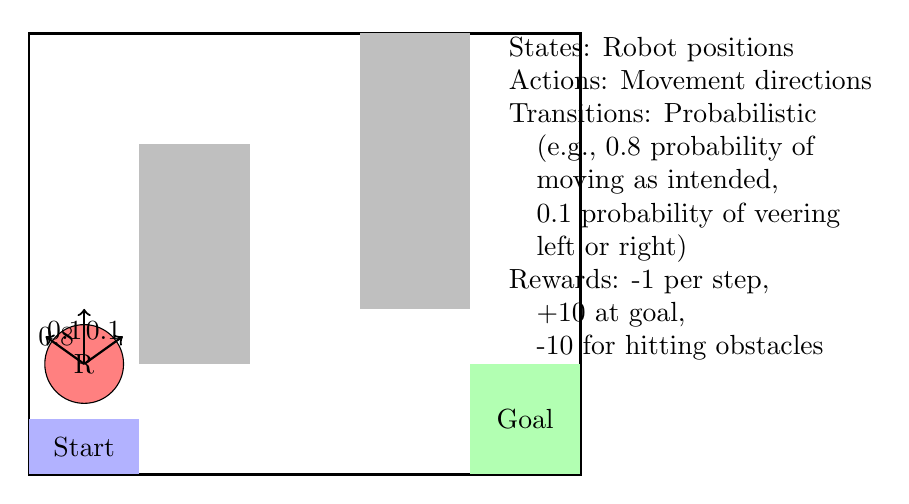
\begin{tikzpicture}[scale=0.7]
    % Draw environment
    \draw[line width=1pt] (0,0) rectangle (10,8);
    
    % Obstacles
    \fill[gray!50] (2,2) rectangle (4,6);
    \fill[gray!50] (6,3) rectangle (8,8);
    
    % Goal
    \fill[green!30] (8,0) rectangle (10,2);
    \node at (9,1) {Goal};
    
    % Start
    \fill[blue!30] (0,0) rectangle (2,1);
    \node at (1,0.5) {Start};
    
    % Robot
    \node[circle, draw, fill=red!50, minimum size=1cm] at (1,2) {R};
    
    % Possible actions and uncertainties
    \draw[->, thick] (1,2) -- (1,3) node[midway, left] {0.8};
    \draw[->, thick] (1,2) -- (1.7,2.5) node[midway, above] {0.1};
    \draw[->, thick] (1,2) -- (0.3,2.5) node[midway, above] {0.1};
    
    % Legend
    \node[align=left] at (12,5) {
    States: Robot positions\\
    Actions: Movement directions\\
    Transitions: Probabilistic\\
    \quad (e.g., 0.8 probability of\\
    \quad moving as intended,\\
    \quad 0.1 probability of veering\\
    \quad left or right)\\
    Rewards: -1 per step,\\
    \quad +10 at goal,\\
    \quad -10 for hitting obstacles
    };
\end{tikzpicture}
\caption{Robot navigation as an MDP}
\end{figure}

\subsection{Resource Management}

MDPs can also model resource allocation problems:

\begin{figure}[H]
\centering
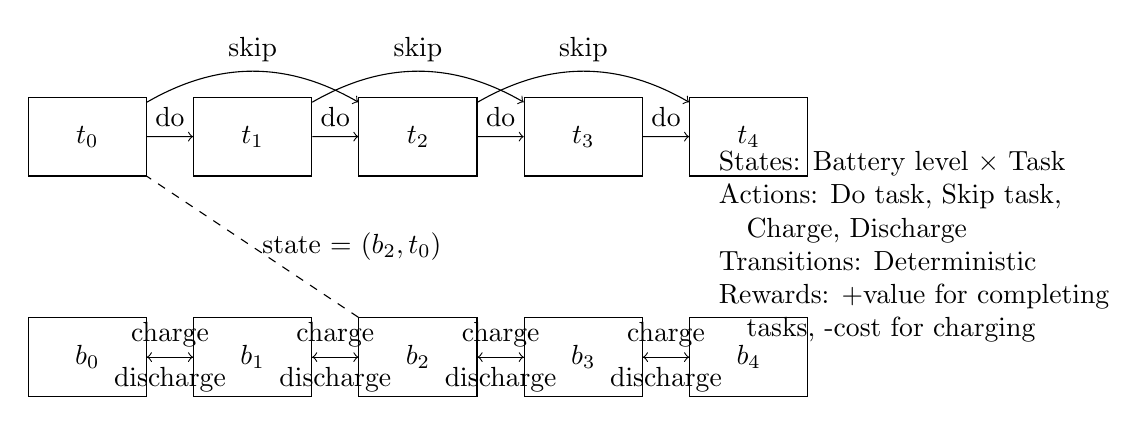
\begin{tikzpicture}[scale=0.7]
    % Draw battery levels
    \node[draw, minimum width=1.5cm, minimum height=1cm] (b0) at (0,0) {$b_0$};
    \node[draw, minimum width=1.5cm, minimum height=1cm] (b1) at (3,0) {$b_1$};
    \node[draw, minimum width=1.5cm, minimum height=1cm] (b2) at (6,0) {$b_2$};
    \node[draw, minimum width=1.5cm, minimum height=1cm] (b3) at (9,0) {$b_3$};
    \node[draw, minimum width=1.5cm, minimum height=1cm] (b4) at (12,0) {$b_4$};
    
    % Battery connections
    \draw[->] (b0) -- (b1) node[midway, above] {charge};
    \draw[->] (b1) -- (b2) node[midway, above] {charge};
    \draw[->] (b2) -- (b3) node[midway, above] {charge};
    \draw[->] (b3) -- (b4) node[midway, above] {charge};
    
    \draw[->] (b1) -- (b0) node[midway, below] {discharge};
    \draw[->] (b2) -- (b1) node[midway, below] {discharge};
    \draw[->] (b3) -- (b2) node[midway, below] {discharge};
    \draw[->] (b4) -- (b3) node[midway, below] {discharge};
    
    % Task states
    \node[draw, minimum width=1.5cm, minimum height=1cm] (t0) at (0,4) {$t_0$};
    \node[draw, minimum width=1.5cm, minimum height=1cm] (t1) at (3,4) {$t_1$};
    \node[draw, minimum width=1.5cm, minimum height=1cm] (t2) at (6,4) {$t_2$};
    \node[draw, minimum width=1.5cm, minimum height=1cm] (t3) at (9,4) {$t_3$};
    \node[draw, minimum width=1.5cm, minimum height=1cm] (t4) at (12,4) {$t_4$};
    
    % Connect task states
    \draw[->] (t0) -- (t1) node[midway, above] {do};
    \draw[->] (t1) -- (t2) node[midway, above] {do};
    \draw[->] (t2) -- (t3) node[midway, above] {do};
    \draw[->] (t3) -- (t4) node[midway, above] {do};
    
    % Skip connections
    \draw[->] (t0) to[bend left=30] node[above] {skip} (t2);
    \draw[->] (t1) to[bend left=30] node[above] {skip} (t3);
    \draw[->] (t2) to[bend left=30] node[above] {skip} (t4);
    
    % Battery-task connections (simplified)
    \draw[dashed] (b2) -- (t0) node[midway, right] {state = $(b_2, t_0)$};
    
    % Legend
    \node[align=left] at (15,2) {
    States: Battery level $\times$ Task\\
    Actions: Do task, Skip task,\\
    \quad Charge, Discharge\\
    Transitions: Deterministic\\
    Rewards: +value for completing\\
    \quad tasks, -cost for charging
    };
\end{tikzpicture}
\caption{Resource management as an MDP}
\end{figure}

\section{Conclusion}

Markov Decision Processes provide the formal mathematical framework for modeling sequential decision-making problems. They extend simpler frameworks like multi-armed bandits by introducing state transitions that are influenced by the agent's actions, allowing for the modeling of long-term consequences.

Key concepts covered in this chapter include:

\begin{itemize}
    \item The four essential components of an MDP: states, actions, transitions, and rewards
    \item The formal MDP definition using mathematical notation and constraints
    \item Policies as mappings from states to action probabilities
    \item Episodic versus continuing tasks and the unification of their notation
    \item The discounting of future rewards and its mathematical and practical justifications
    \item Value functions and their recursive relationships expressed in the Bellman equations
    \item Optimal policies and value functions characterized by the Bellman optimality equations
    \item Various methods for solving MDPs to find optimal policies
\end{itemize}

Understanding MDPs is crucial for reinforcement learning, as they provide the theoretical foundation upon which algorithms are built. The concepts of value functions, policies, and the Bellman equations are fundamental to virtually all reinforcement learning methods, from classic techniques like dynamic programming to modern approaches based on deep neural networks.

\end{document}
